\documentclass[10pt]{beamer}

\usetheme[progressbar=frametitle]{metropolis}
\usepackage{appendixnumberbeamer}

\usepackage[autoplay]{animate}
\usepackage{graphicx}

\usepackage{booktabs}
\usepackage[scale=2]{ccicons}

%\usepackage{pgfplots}
%\usepgfplotslibrary{dateplot}

\usepackage{xspace}

\setbeamercolor{normal text}{bg=white}
\newcommand{\themename}{\textbf{\textsc{metropolis}}\xspace}

\title{Examining Hausdorff dimension and Scaling behaviour with Worm algorithm}
%\subtitle{A modern beamer theme}
\date{\today}
\date{}
\author{Simon Rydell}
\institute{Royal Institute of Technology, Stockholm}
% \titlegraphic{\hfill\includegraphics[height=1.5cm]{logo.pdf}}

\begin{document}

\maketitle

\begin{frame}{Table of contents}
  \setbeamertemplate{section in toc}[sections numbered]
  \tableofcontents[hideallsubsections]
\end{frame}

\section{Fractals}

\begin{frame}{Scaling Mass}
    hi
\end{frame}

\begin{frame}{A Measure of Roughness}
    hi
\end{frame}

\begin{frame}{Box Counting Method}
    hi
\end{frame}

\begin{frame}{Hausdorff Dimension}
    hi
\end{frame}

\section{Algorithms Used For Generating Graph Patterns}

\begin{frame}{Worm Algorithm}
    Idea is to sample non-zero contributions of the partition function at $T = T_c$. Express them in a way as to form `loops'.
\end{frame}

\begin{frame}{Hoshen Kopelman Labeling and Graph Dividing}
    Idea is to sample non-zero contributions of the partition function at $T = T_c$. Express them in a way as to form `loops'.
\end{frame}

\section{Ising Model}

\begin{frame}{Ising Loop Expansion}
    hi
\end{frame}

\begin{frame}{Box Dimension}
    \begin{figure}[h!]
        \centering
            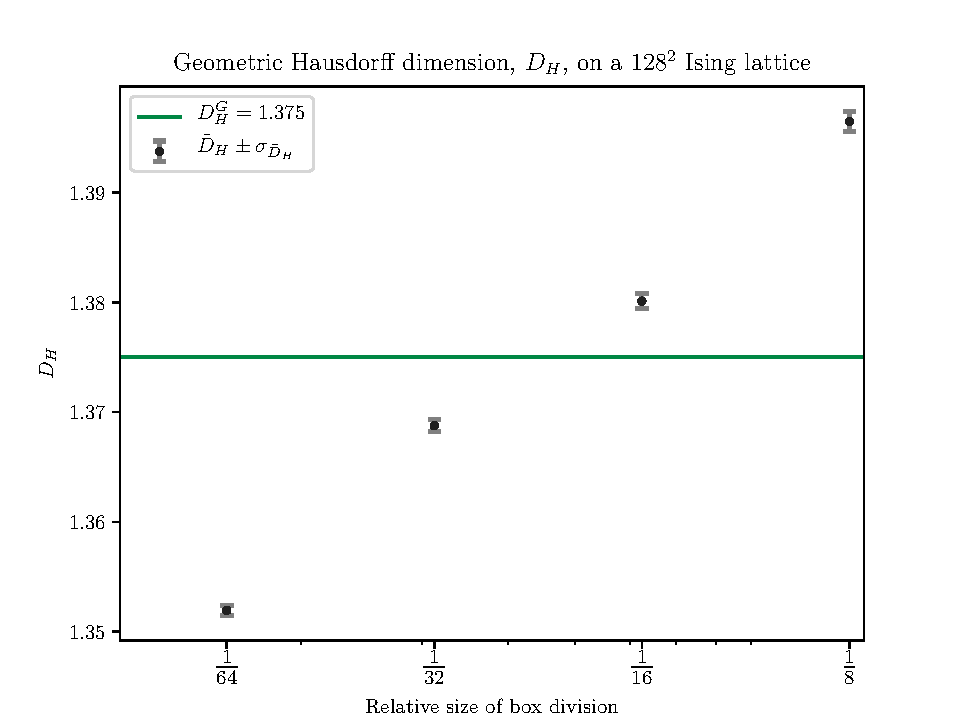
\includegraphics[width=0.8\textwidth]{figures/box_dim_128x128Ising.pdf}
    %    \caption{}
    %    \label{fig:}
    \end{figure}
\end{frame}

\begin{frame}{Scaling Dimension}
    \begin{figure}[h!]
        \centering
            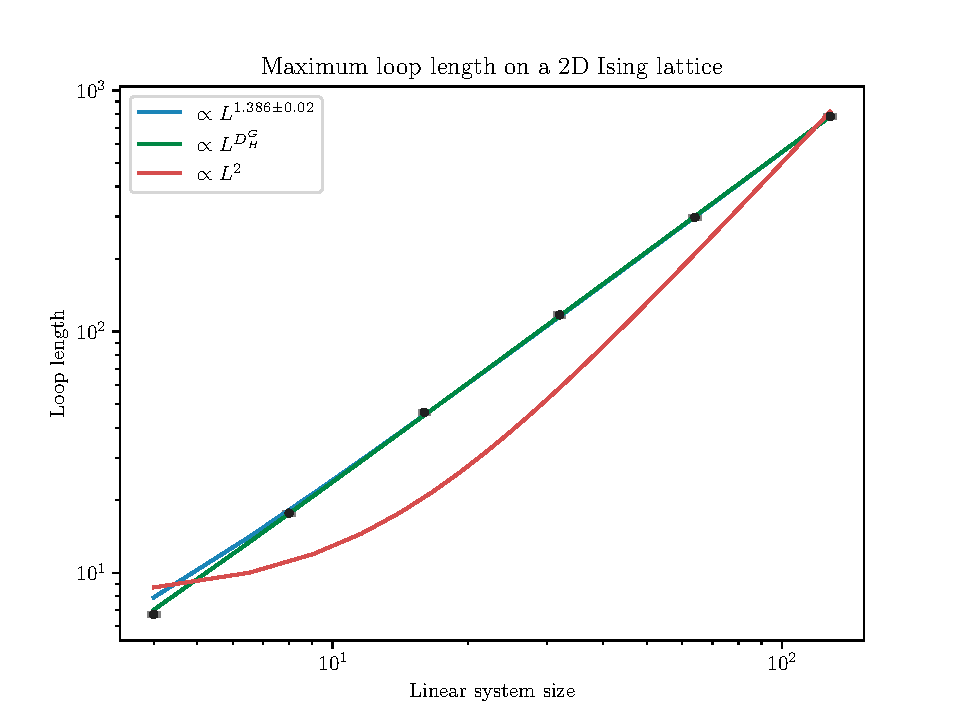
\includegraphics[width=0.8\textwidth]{figures/maximum_loop_length_for_2D_Ising.pdf}
    %    \caption{}
    %    \label{fig:}
    \end{figure}
\end{frame}

\begin{frame}{Comparison of Dimensions $2D$ Ising}
    \begin{figure}[h!]
        \centering
            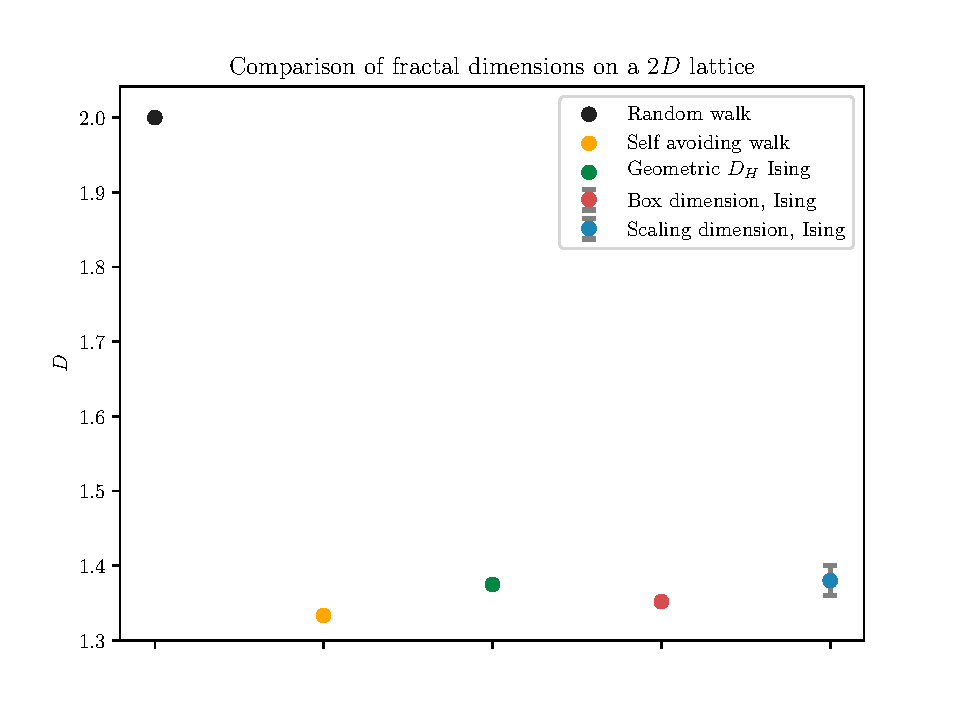
\includegraphics[width=0.8\textwidth]{figures/dimenson_comparison.pdf}
    %    \caption{}
    %    \label{fig:}
    \end{figure}
\end{frame}


\begin{frame}{$2D$ Ising Animation}
    % TODO: Uncomment
    %  \animategraphics[width=\linewidth,loop]{10}{figures/2dising_animation}{}{}
\end{frame}

\begin{frame}{Largest Ising Loop on a $128^2$ Lattice}
    \begin{figure}[h!]
        \centering
            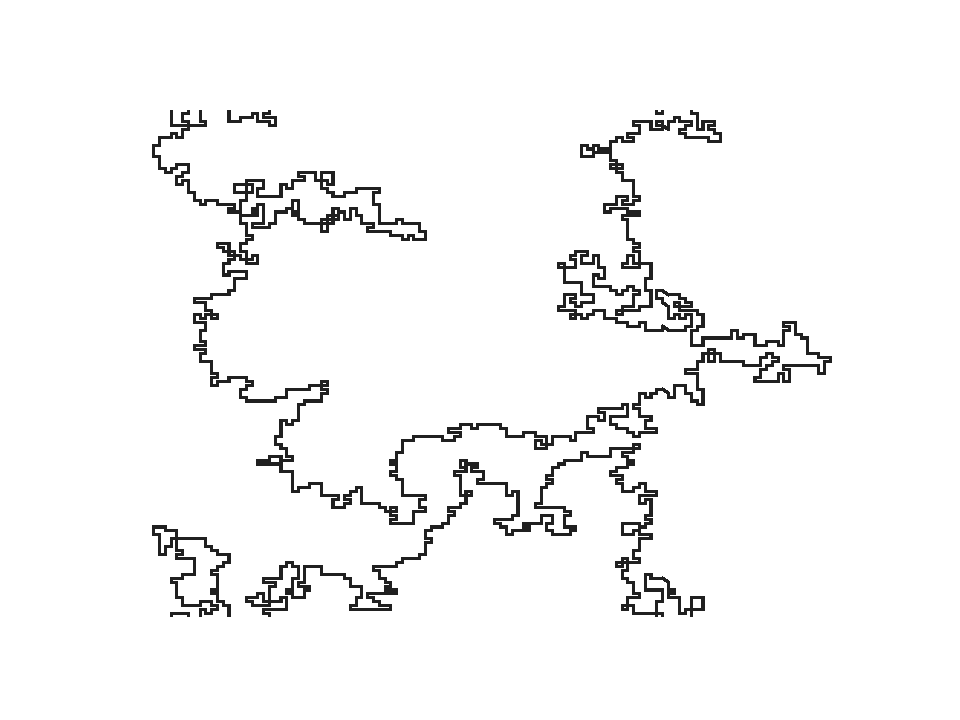
\includegraphics[width=0.8\textwidth]{figures/largest_cluster_testing_nolattice.pdf}
    %    \caption{}
    %    \label{fig:}
    \end{figure}
\end{frame}

\section{XY Model}

\begin{frame}{XY Model}
    Rotors... Loop Expansion. Adds complexity as a direction and weight. Use Villain approximation $\Rightarrow$ Displaces $T_c$ $\Rightarrow$ Use winding number to `find' $T_c$.
\end{frame}

\begin{frame}{Winding Number}
    Explain how winding numbers can show $T_c$. Maybe illustrations.
\end{frame}

\begin{frame}{Winding Number}
    \begin{figure}[h!]
        \centering
            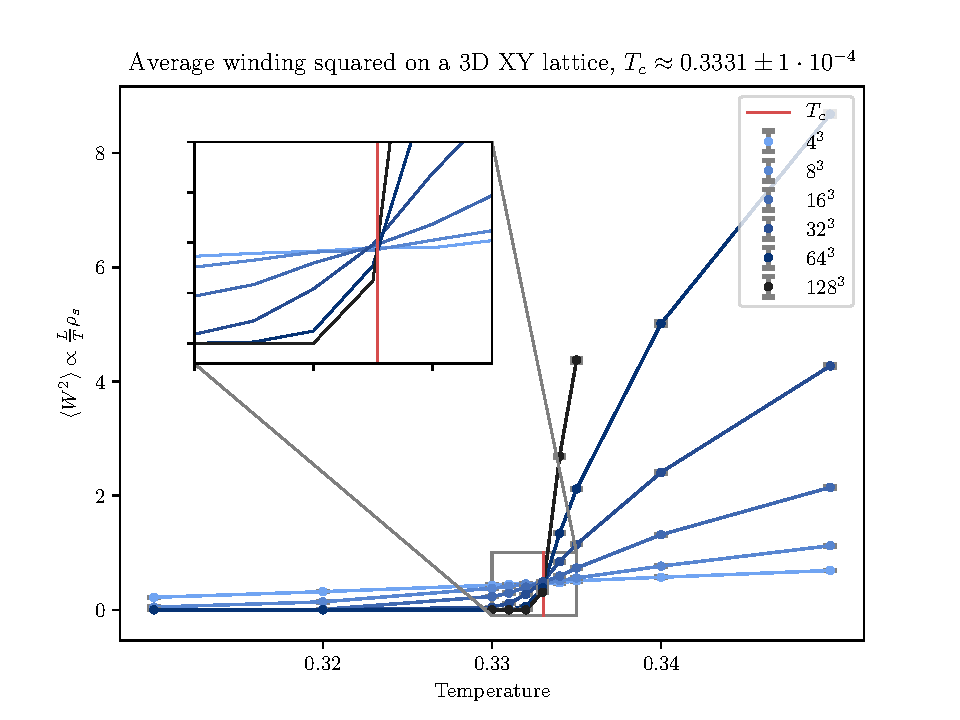
\includegraphics[width=0.8\textwidth]{figures/winding_number_Tc_zoomed.pdf}
    %    \caption{}
    %    \label{fig:}
    \end{figure}
\end{frame}

\begin{frame}{$3D$ XY Model Hausdorff Dimension}
    \begin{enumerate}[$\bullet$]
        \item Hove, Mo and Sudbo: $D_H = 2.287 \pm 2 \cdot 10^{-3}$
        \item Prokof'ev and Svistunov Comment: $D_H = 1.7655 \pm 2 \cdot 10^{-3}$
    \end{enumerate}
\end{frame}

\begin{frame}{Box Counting Method $3D$ XY}
    \begin{figure}[h!]
        \centering
            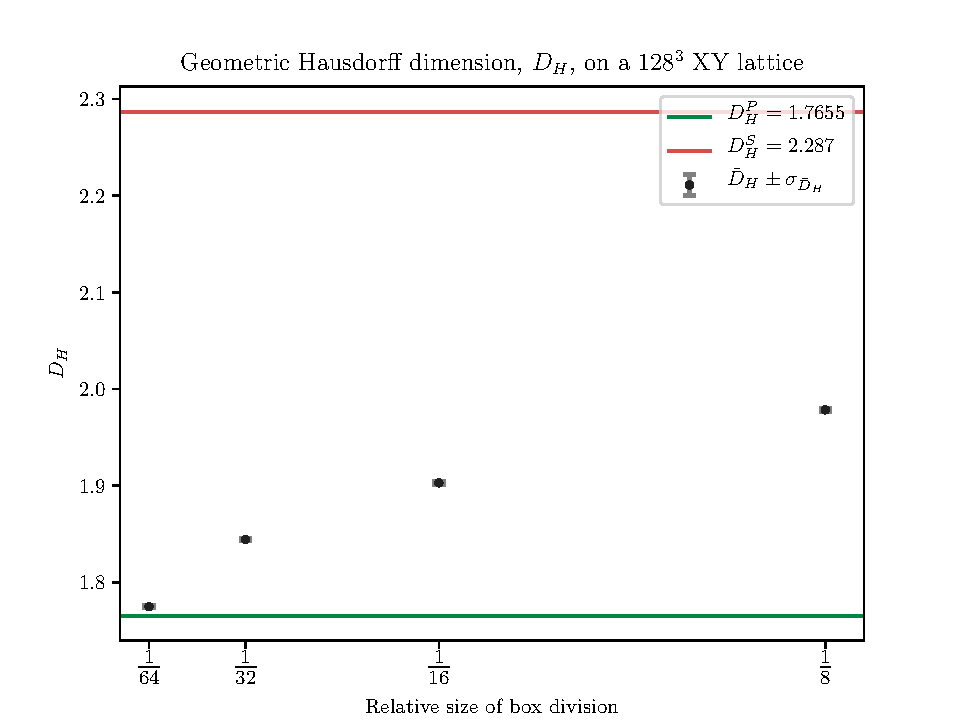
\includegraphics[width=0.8\textwidth]{figures/box_dimension_xy_128x3.pdf}
    %    \caption{}
    %    \label{fig:}
    \end{figure}
\end{frame}

\begin{frame}{Comparison of Dimensions $3D$ XY}
    \begin{figure}[h!]
        \centering
            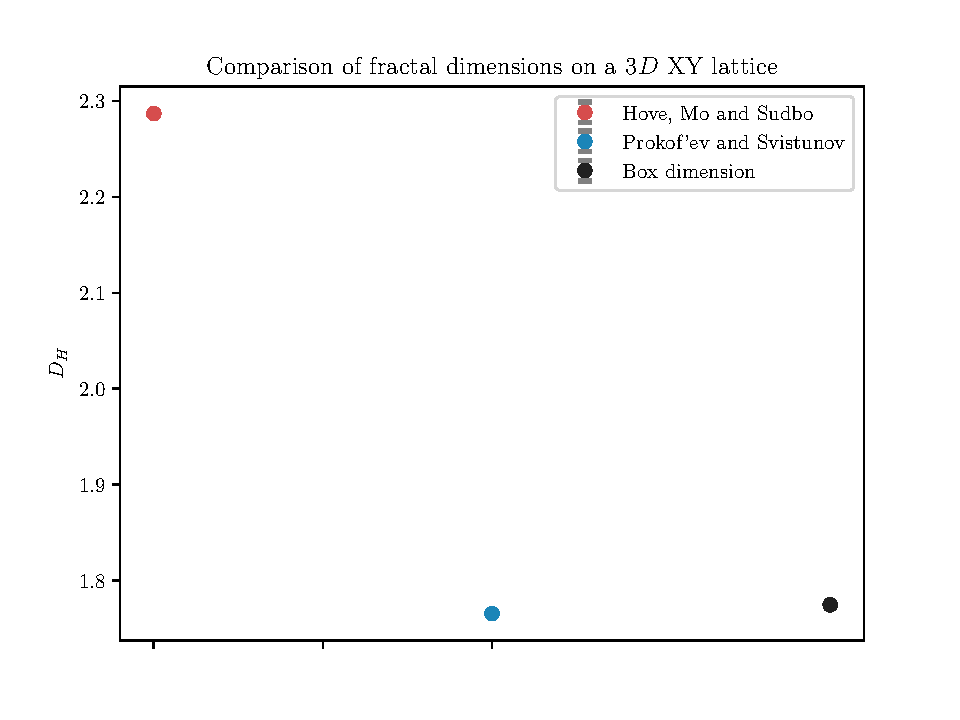
\includegraphics[width=0.8\textwidth]{figures/dimenson_comparison_XY.pdf}
    %    \caption{}
    %    \label{fig:}
    \end{figure}
\end{frame}


\begin{frame}{$3D$ XY Animation}
%  \animategraphics[width=\linewidth,loop]{10}{figures/3dxy_animation}{}{}
\end{frame}

\begin{frame}{Summary}
    \begin{table}
        \parbox{.45\linewidth}{
            \centering
            \begin{tabular}{l|l}
                               & $D_H$          \\ \hline
                Box            & $1.35193(5)$   \\ \hline
                Scaling        & $1.38(2)$      \\ \hline
                $D_H^G$        & $1.375$        \\ \hline
                SAW            & $1.33$         \\ \hline
                Random Walk    & $2$                          
            \end{tabular}
            \caption{$2D$ Ising}
        }
        \hfill
        \parbox{.45\linewidth}{
            \centering
            \begin{tabular}{l|l}
                            & $D_H$           \\ \hline
                Box         & $1.77468(4)$    \\ \hline
                Prokof'ev   & $1.765(2)$      \\ \hline
                Sudbo       & $2.287(2)$  
            \end{tabular}
            \caption{$3D$ XY}
        }
    \end{table}
\end{frame}


\end{document}